%
% ultima actualizare: Mihai Popescu - 03/03/2020

\section{Experimente practice}

\subsection*{Aparate, componente 'si software necesar}

Pachetul ({\em kit}-ul) de laborator pe care 'il ve'ti primi con'tine: 
\begin{itemize}
\item o unitate multifunc'tional'a ANALOG DISCOVERY 2 (Fig.~\ref{fig:4_AD2_multi}, st\^anga) \cite{ad2_refman}; unitatea va fi utilizat'a ca surs'a de tensiune variabil'a 'si voltmetru;
\item un multimetru digital (Fig.~\ref{fig:4_AD2_multi}, dreapta) \cite{multimeter_manual}. Acest aparat va fi folosit pentru m'asurarea curen'tilor 'si a rezisten'telor;
\item o plac'a de test ({\em breadboard}) pe care se va executa montajul experimental, conform schemelor electrice descrise 'in lucrare;
\item un set de rezistoare din care se vor selecta doar cele necesare rezolv'arii cerin'telor lucr'arii.
\end{itemize}
'In plus, ave'ti nevoie de
\begin{itemize}
\item interfa'ta software "WaveForms" ce reprezint'a setul de instrumente virtuale asociat unit'a'tii ANALOG DISCOVERY 2 \cite{wavef_refman} ; 
\item software de simulare a circuitelor electrice - LTspice \cite{ltspice};
\item o foaie de calcul electronic'a (MsExcel, OpenOffice Calc, etc.).
\end{itemize}
\begin{figure}
	\centering
		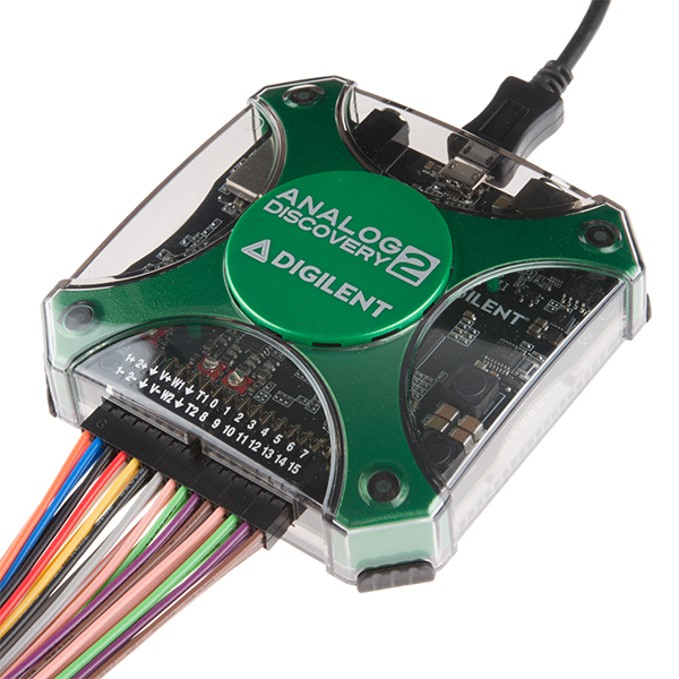
\includegraphics[width=0.4\textwidth]{laborator_01/figuri/4_AD2.jpg}
		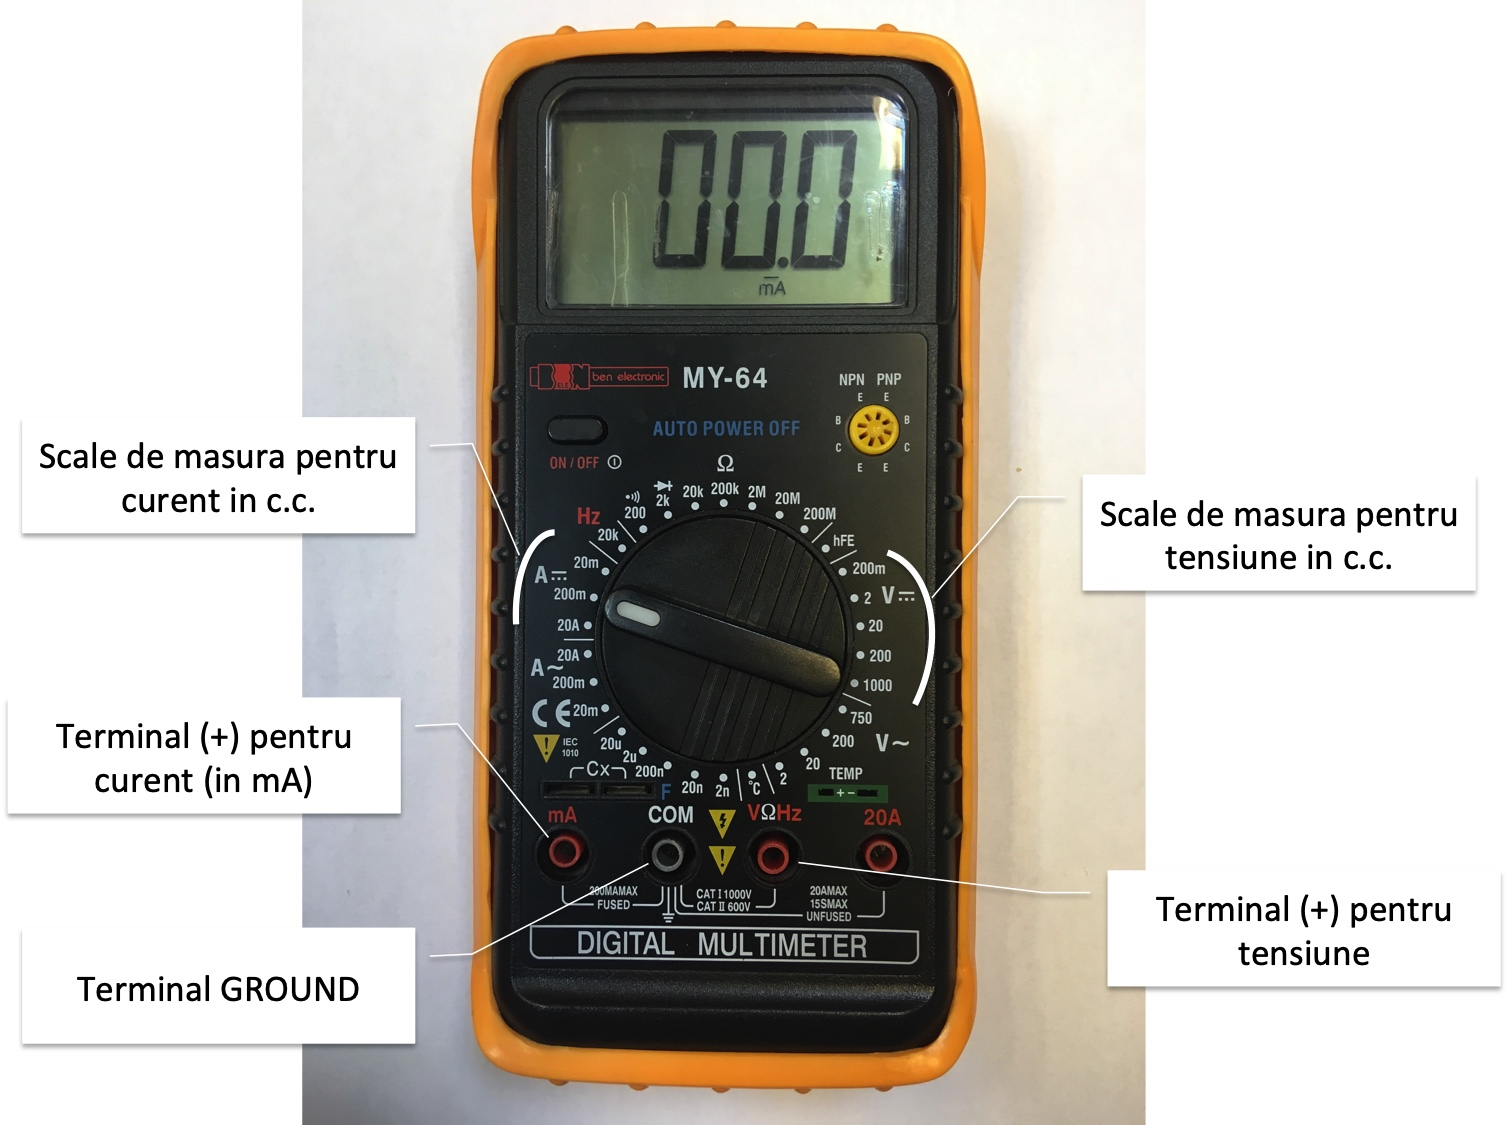
\includegraphics[width=0.5\textwidth]{laborator_01/figuri/4_multimetru_prel}
	\caption{Unitatea multifunc'tional'a ANALOG DISCOVERY 2 (st\^anga) 'si multimetrul (dreapta).}
	\label{fig:4_AD2_multi}
\end{figure}
%
%
\subsection*{Lucrarea de laborator -- pas cu pas}

Experimentele pe care trebuie s'a le realiza'ti sunt descrise mai jos. 'In paralel cu ele trebuie s'a completa'ti chestionarul corespunz'ator de pe platforma Moodle.

 \textbf{\color{red} Aten'tie!} Acest chestionar 'il pute'ti completa o singur'a dat'a, 'in timpul laboratorului. 

Deschide'ti chestionarul de pe moodle 'si 'incepe'ti a-l completa strict 'in ordinea apari'tiei problemelor de abordat. Este important'a p'astrarea acestei ordini 'intruc\^at rezultatele ob'tinute la un moment dat vor folosi pentru etape urm'atoare ale aceluia'si chestionar. 

\textbf{\color{red} Acest chestionar este un "formular de lucru" care trebui  completat pas cu pas.}

\begin{exercise}[Pasul 1. Deschiderea chestionarului 'si rezolvarea chestiunilor teoretice.]
	Deschide'ti chestionarul de pe moodle 'si  r'aspunde'ti la primele 'intreb'ari care se refer'a la teoria lucr'arii.
\end{exercise}

Fiecare student deschide un astfel de chestionar. 'Intreb'arile teoretice primite sunt, 'in general, diferite. Pute'ti lucra 'in echip'a pentru a decide r'aspunsurile corecte.

%
% -------------- Q1 ----------------
%
\begin{exercise}[Pasul 2. Preg'atirea componentelor.]
	'Inaintea 'inceperii p'ar'tii practice a oric'arei lucr'ari de laborator este necesar'a inventarierea componentelor cu care se va realiza montajul experimental. 'In acest scop va trebui s'a determina'ti, pe baza codului culorilor (Fig.~\ref{fig:rezistente_cod_culori}), valorile rezisten'telor 'inscrise pe corpurile rezistoarelor din kit-ul primit. Pentru validarea corectitudinii citirilor pute'ti folosi func'tia de ohmetru a multimetrului digital. Constata'ti faptul c'a valorile m'asurate difer'a de cele 'inscrise prin codul culorilor, 'in limita toleran'tei de fabrica'tie  indicat'a tot printr-o culoare.  
\end{exercise}
%\todoINFO{Aici ar trebui o referin't'a c'atre ecua'tiile care dau marginile erorii absolute care NU sunt etichetate inc'a}
\begin{observ}
	Pe foaia de calcul electronic'a pute'ti verifica, pentru fiecare rezistor, 'inscrierea valorii determinate cu ohmetrul 'in limitele toleran'tei specificate pe corpul rezistorului prin cod de culoare; verificarea se poate face prin implementarea, pe foaia de calcul electronic'a, a rela'tiilor din capitolul dedicat propag'arii erorilor. 
\end{observ}
%
\begin{figure}
	\centering
		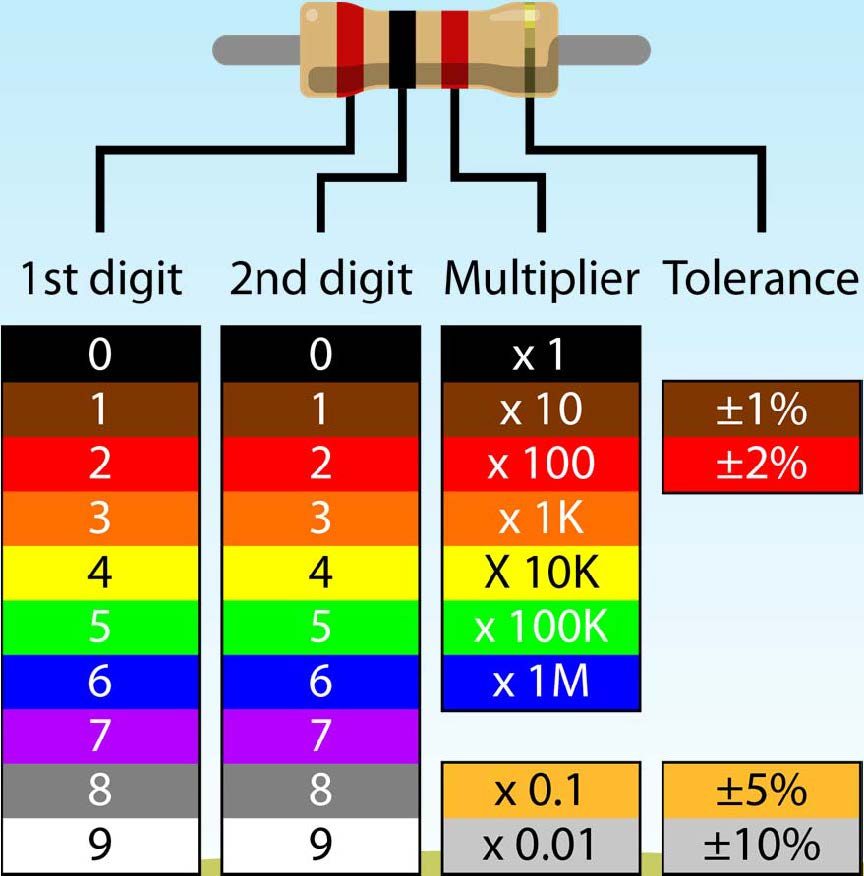
\includegraphics[width=0.4\textwidth]{laborator_01/figuri/rezistente_cod_culori}
	\caption{Codul de culori pentru un rezistor are 4 benzi. Primele dou'a benzi indic'a primele dou'a cifre semnificative, iar a treia band'a reprezinta puterea lui 10 cu care se multiplic'a num'arul 'intreg de 2 cifre codificat de primele dou'a benzi. A patra band'a reprezinta toleran'ta 'in procente. Valoarea rezisten'tei din figur'a este de $20 \cdot 10^2 \, \Omega = 2 \, k\Omega$, cu o toleran't'a de 5\%. Pe scurt: $2 \, k\Omega \pm 5\%$.}
	\label{fig:rezistente_cod_culori}
\end{figure}
%
% ------------------ Q2 -----------------
%
\begin{exercise}[Condi'tii de proiectare a circuitului] \label{Q2}
Din setul de rezistoare primite selecta'ti-le pe cele care v'a permit realizarea unui divizor cu  un raport $k = U_1/U_2$ indicat 'in enun'tul exerci'tiului. Alegerea trebuie s'a fie f'acut'a astfel 'inc\^at curentul prin divizor s'a nu fie mai mic de o valoare  $I_{\mathrm{div}_{\mathrm{min}}}$   indicat'a 'in formular. 
\end{exercise}
%
\begin{indicatie}
Determina'ti mai 'int\^ai rezisten'ta total'a maxim'a a divizorului din rela'tia 
\begin{equation} \label{rdivmax}
	(R_1 + R_2)\leq U_1/I_{\mathrm{div}_{\mathrm{min}}}.
\end{equation}
 'In continuare, utiliz\^and rela'tiile \eqref{retine1}, determina'ti raportul dintre cele dou'a rezisten'te, imediat rezult\^and 'si valorile teoretice pentru fiecare dintre ele. 'In final nu r'am\^ane dec\^at s'a selecta'ti, din setul disponibil, rezistoarele care au cele mai mari rezisten'te apropiate de valorile teoretice determinate, dar mai mici dec\^at acestea, a.'i. s'a fie satisf'acut'a condi'tia \eqref{rdivmax}. 
\end{indicatie}
%
% ---------------- Q3 -----------------
%
\begin{exercise}[Verificarea teoretic'a a circuitului proiectat] \label{Q3}
Aplic\^and rela'tia \eqref{eq:tensiune_intrare_gol}, determina'ti valorile curentului prin divizorul de tensiune $I_{\mathrm{div}}$, respectiv a tensiunii $U_2$ de la ie'sirea acestuia, 'in condi'tiile 'in care tensiunea de intrare este cea specificat'a la exerci'tiul \ref{Q2}. Pentru $R_1$, respectiv $R_2$ folosi'ti valorile rezisten'telor alese 'in acela'si exerci'tiu.  
\end{exercise}
%
% ---------------- Q4 -----------------
%
\begin{exercise} [Simularea unui model virtual al circuitului proiectat] \label{Q4}
Folosind una din tehnicile descrise 'in sec'tiunea  \ref{sec:ltspice}, conform 
Fig.~ \ref{fig:spice_ex1_3} 'si/sau Fig.~\ref{fig:spice_ex1_4}, simula'ti func'tionarea 'in gol a divizorului de tensiune, cu valorile date, respectiv determinate la exerci'tiul \ref{Q2}. Completa'ti formularul de lucru cu rezultatele ob'tinute din simulare.
\end{exercise}
%
% ---------------- Q5 -----------------
%
\begin{exercise} [Realizarea circuitului pe placa de test 'si verificarea parametrilor func'tionali la mersul 'in gol] \label{Q5}
Pentru a efectua cu u'surin't'a procedurile de m'asurare ce vor urma, precum 'si pentru a reduce posibilit'a'tile de a gre'si, este foarte important s'a desena'ti pe h\^artie schema divizorului, etichet\^and fiecare nod de circuit cu num'arul nodului corespunz'ator de pe placa de test. 'In acest mod ve'ti putea:
\begin{itemize}
\item detecta cu u'surin't'a eventuale erori de montaj;
\item stabili clar noduri importante utile pentru a m'asur'a curen'ti, tensiuni, poten'tiale;
\item urm'ari 'in mod coerent 'si ordonat toate modific'arile pe care le ve'ti opera 'in topologia circuitului experimental.  
\end{itemize}
%
O recomandare a unei posibile a'sez'ari (poz'ari) a componentelor este dat'a 'in Fig.~\ref{fig:4_divizor1_bb}. Tensiunea de intrare $U_1$ este asigurat'a din sursa de tensiune continu'a pozitiv'a a unit'a'tii AD2, 'intre bornele $V+$ 'si $\mathrm{GND}$. Pentru determinarea curentului prin divizorul de tensiune, conecta'ti multimetrul (setat pe func'tia 200mA/cc) 'in serie cu gruparea $R_1 - R_2$. Pentru m'asurarea tensiunii $U_2$, folosi'ti primul canal de m'asur'a al AD2 'intre bornele $+1$ 'si $-1$.
\begin{retine}
	{\color{blue}
Orice modificare 'in schem'a se va efectua fie cu portul USB al AD2 deconectat, fie cu sursele de tensiune oprite 
("MASTER ENABLE" - 'in stare $\mathrm{OFF}$).
}
\end{retine}
Pentru efectuarea montajului 'si a m'asur'arilor urma'ti urm'atorii pa'si:
\begin{enumerate}
\item Asigura'ti-v'a c'a AD2 are cablul USB deconectat din calculator;
\item Realiza'ti montajul experimental conform schemei;  
\item Verifica'ti corectitudinea conexiunilor (coresponden'ta dintre schem'a 'si montaj); dac'a nu sunte'ti siguri pe ce a'ti realizat practic, discuta'ti cu profesorul 'indrum'ator;
\item Conecta'ti cablul AD2 'in portul USB al calculatorului;
\item Lansa'ti panoul virtual de instrumente al AD2 din meniul \textit{Windows $->$ Digilent $->$ WaveForms};
\item Dup'a ce interfa'ta porne'ste, se va conecta automat la AD2; acest lucru este confirmat de o diod'a luminiscent'a (LED) care se aprinde intermitent 'in unitatea AD2;
\item Deschide'ti interfa'ta voltmetrului - $Voltage$ 'si activa'ti-o cu "click" pe butonul $Run$;
\item Deschide'ti interfa'ta surselor de tensiune ("Supplies") 'si 'in fereastra \textit{Voltage} a primei surse, seta'ti tensiunea $U_1$ la valoarea indicat'a la exerci'tiul \ref{Q2};
\item Activa'ti sursa de tensiune prin "click" pe \textit{"Positive Supply (V+) Rdy"}, iar apoi pe \textit{"Master Enable"} care din starea OFF va trece 'in starea ON.
\item Dac'a totul este corect, pe afi'sajul DC al voltmetrului 1 va ap'area tensiunea $U_2$, iar pe afi'sajul multimetrului va ap'area intensitatea curentului prin divizor.
\item Cele dou'a valori trebuie s'a fie apropiate de valorile determinate din ecua'tii 'si prin simulare cu LTspice; dac'a acest lucru nu se 'int\^ampl'a, verifica'ti din nou corectitudinea montajului, respectiv valorile componentelor utilizate;
\item Verifica'ti dac'a intensitatea curentului prin divizor este mai mare sau egal'a cu $I_{\mathrm{div}_{\mathrm{min}}}$;
\item {\color{blue}{Pentru determinarea cu precizie bun'a a tensiunii de ie'sire $U_2$, elimina'ti ampermetrul din circuit, 'intruc\^at rezisten'ta sa intern'a modific'a raportul de divizare a divizorului de tensiune}};
\item Nota'ti pe formularul de lucru valorile m'asurate;
\item Dezactiva'ti sursa de alimentare (\textit{"Master Enable"} 'in stare OFF). 
\end{enumerate}
\end{exercise}
%

\begin{observ}
		\begin{itemize}
			\item 	{\color{blue}
				Orice modificare 'in schem'a se va efectua fie cu portul USB al AD2 deconectat, fie cu sursele de tensiune oprite 
				("MASTER ENABLE" - 'in stare $\mathrm{OFF}$).}
\item nota'ti-v'a pe foaia de calcul electronic'a rezultatele m'asur'arilor;
\item ca schem'a de referin't'a, 'in loc de schema pe h\^artie, pute'ti folosi 'si schema generat'a cu interfa'ta grafic'a a LTspice, cu condi'tia de a eticheta 'si acolo nodurile (butonul \textit{Label Net}) cu acelea'si etichete numerice ca ale nodurilor corespunz'atoare de pe placa de test.
\end{itemize} 
\end{observ}
%
\begin{figure}
	\centering
		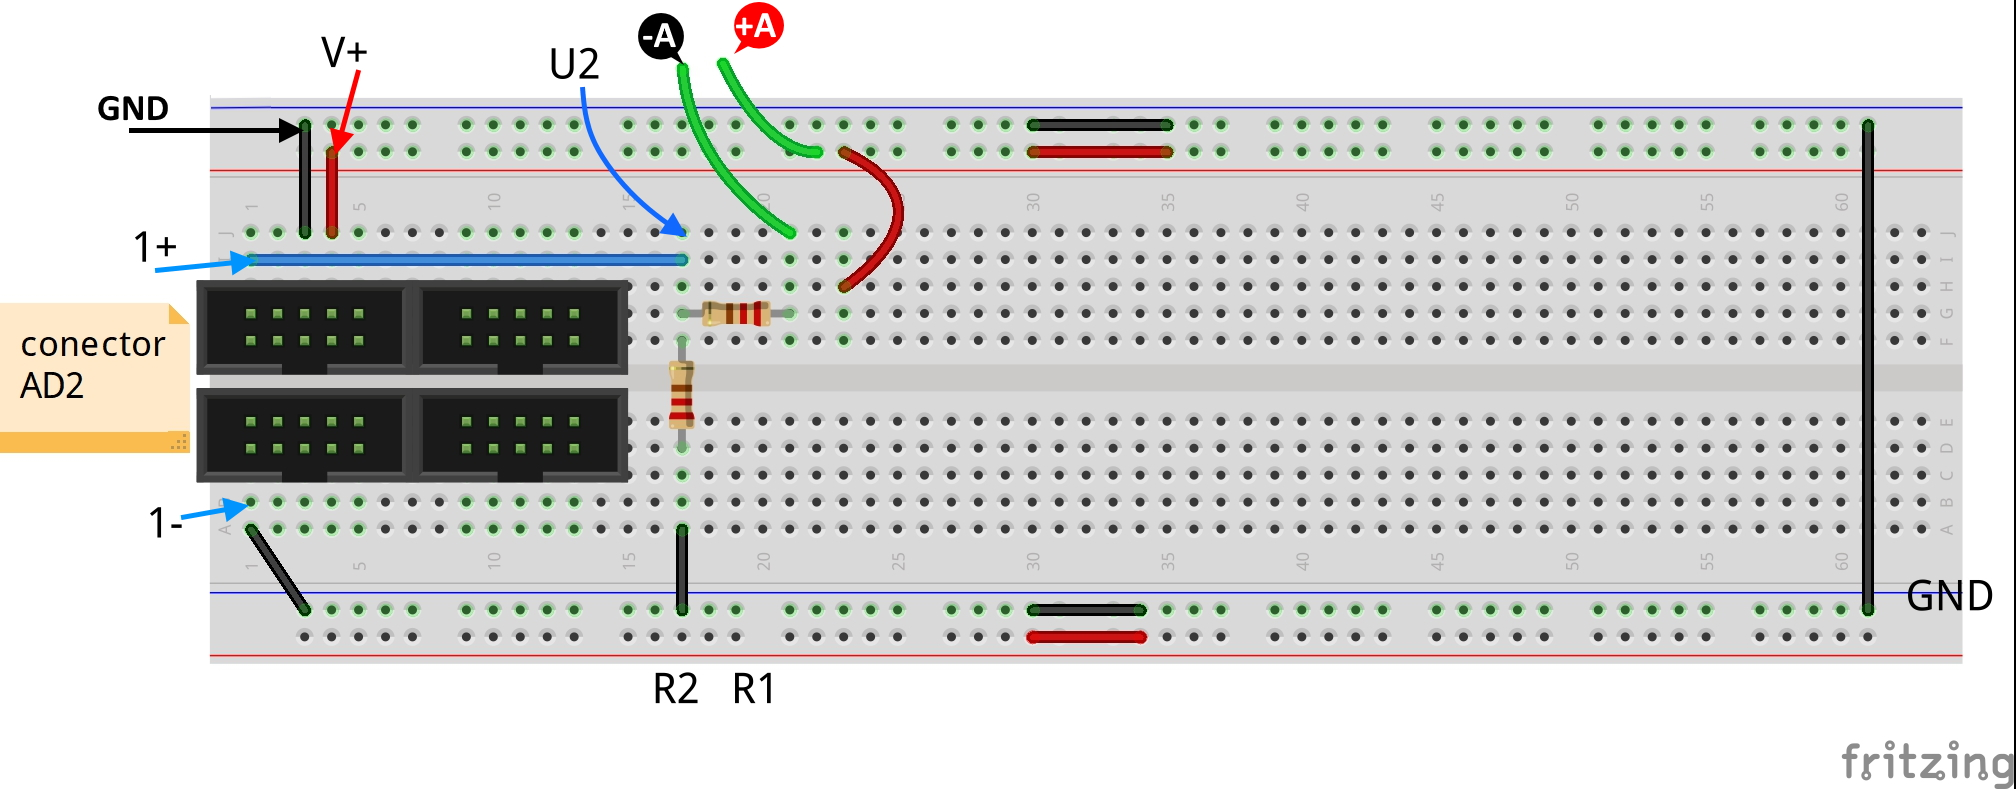
\includegraphics[width=0.8\textwidth]{laborator_01/figuri/4_divizor_1_bb}
	\caption{Amplasamentul componentelor pentru divizorul de tensiune. Curentul se m'asoar'a conect\^and multimetrul pe scara de mA/cc 'intre bara de alimentare V+ (ro'sie) 'si R1. Tensiunea se m'asoar'a prin canalul de m'asur'a 1 al AD2, conect\^and intrarea 1- la bara GND (albastr'a), 'si intrarea 1+ la ie'sirea divizorului de tensiune.}
	\label{fig:4_divizor1_bb}
\end{figure}
%
% ---------------- Q6 -----------------
%
\begin{exercise}[Stabilirea modului de testare a circuitului 'in sarcin'a] \label{Q6}
	Determina'ti rezisten'ta de sarcin'a $R_s$, astfel 'inc\^at $I_s \leq 50 \cdot I_{\mathrm{div}}$. Unde pentru $I_{div}$ considera'ti valoarea m'asurat'a la exerci'tiul \eqref{Q5}. \c{T}ine'ti cont c'a rezisten'ta are o toleran't'a de $\pm 5\%$.	
\end{exercise}
%
\begin{indicatie}
	Pentru determin'arile de mai jos, folosi'ti foaia electronic'a de calcul.
	Calcula'ti mai 'int\^ai limita inferioar'a teoretic'a a rezisten'tei de sarcin'a din condi'tia:
\begin{equation} \label{conditie_Rs}
	 R_s \geq 50 \cdot I_{\mathrm{div}_{\mathrm{masurat}}}.
\end{equation}
Determina'ti apoi valoarea teoretic'a ce ar putea fi 'inscris'a pe un rezistor cu toleran't'a $\pm 5\%$ astfel ca, 'in cel mai defavorabil caz, condi'tia \eqref{conditie_Rs} s'a fie respectat'a.
\end{indicatie}
%
% ---------------- Q7 -----------------
%
\begin{exercise}[Testarea circuitului 'in sarcin'a] \label{Q7} %, conform modului de testare stabilit] \label{Q7}
	Alege'ti rezistorul, cu cea mai mic'a valoare de rezisten't'a, disponibil 'in kit-ul primit, care 'indepline'ste condi'tia impus'a 'in exerci'tiul \eqref{Q6}. Determina'ti intensitatea curentului de sarcin'a teoretic folosind pentru rezisten't'a valoarea 'inscris'a pe rezistorul ales:
\begin{equation} \label{is_teoretic}
	I_{s_{\mathrm{teoretic}}} = U_{2_{\mathrm{masurat}}} / R_{s_{\mathrm{real}}}.
\end{equation}
	Conecta'ti rezistorul de sarcin'a ales, la ie'sirea divizorului deja construit.  M'asura'ti curentul de sarcin'a $I_{s_{\mathrm{masurat}}}$ 'si calcula'ti eroarea relativ'a fa't'a de valoarea teoretic'a determinat'a. Efectua'ti aceea'si compara'tie 'si pentru tensiunea de ie'sire $U_2$. Selecta'ti ('in formularul de lucru) gama de valori corespunz'atoare erorilor relative ob'tinute pentru cele dou'a m'arimi.	
\end{exercise}
%
\begin{observ}
$I_s$ se m'asoar'a cu multimetrul setat pe scala de m'asur'a 2 mA/cc, respectiv tensiunea cu ajutorul canalului de m'asur'a 1 al AD2;
\begin{itemize}
	\item 	{\color{blue}
		Orice modificare 'in schem'a se va efectua fie cu portul USB al AD2 deconectat, fie cu sursele de tensiune oprite 
		("MASTER ENABLE" - 'in stare $\mathrm{OFF}$).}
\item {\color{blue} Este deosebit de important s'a respecta'ti procedurile de lucru indicate la exerci'tiul \ref{Q5}; }  
\item Nota'ti-v'a pe foaia de calcul electronic'a rezultatele m'asur'arilor;
\end{itemize}
\end{observ}
%
\begin{indicatie}
'In Fig.~\ref{fig:4_divizor_sarcina} este recomandat'a o posibil'a dispunere a componentelor pentru m'asur'arile propuse. {\color{blue} De ce, 'in acest caz, nu este neap'arat necesar'a eliminarea ampermetrului atunci c\^and se m'asoar'a tensiunea de ie'sire $U_2$?}
\end{indicatie}
%
\begin{figure}
	\centering
		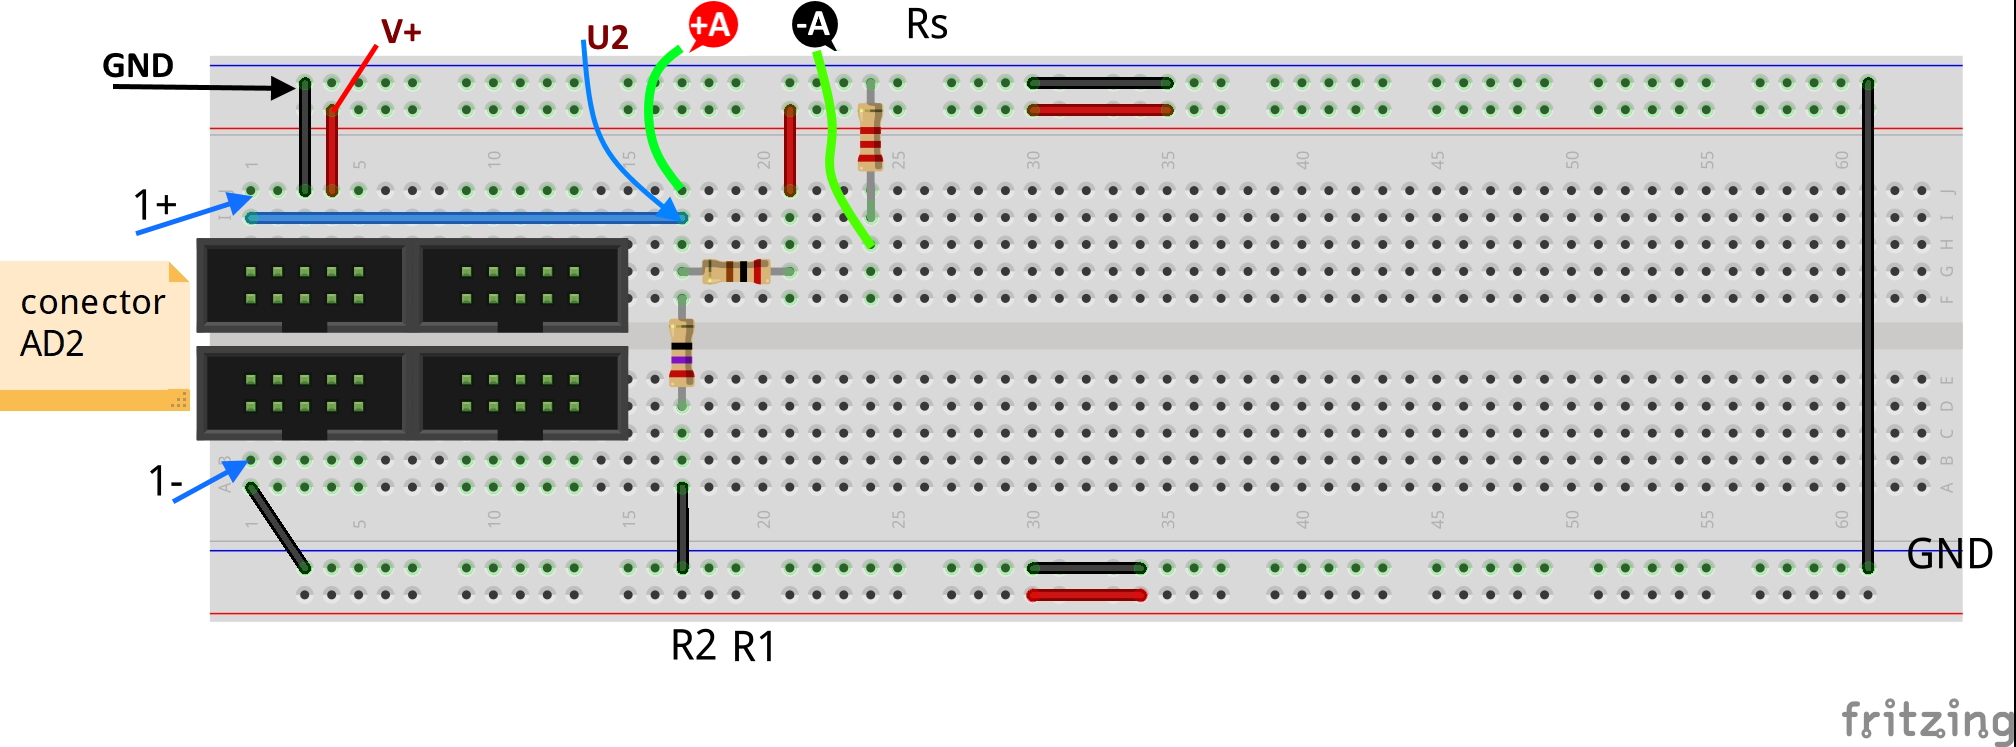
\includegraphics[width=0.8\textwidth]{laborator_01/figuri/4_divizor_sarcina_bb}
	\caption{Montaj pentru m'asurarea parametrilor electrici de ie'sire ai divizorului de tensiune 'in sarcin'a.}
	\label{fig:4_divizor_sarcina}
\end{figure}
%
% ---------------- Q8 -----------------
%
\begin{exercise} [Simularea unui model virtual al circuitului la func'tionarea 'in sarcin'a] \label{Q8}
Folosind una din tehnicile descrise 'in sec'tiunea  "LTspice", conform Fig.~\ref{fig:spice_ex1_3} 'si/sau Fig.~\ref{fig:spice_ex1_4}, simula'ti func'tionarea 'in sarcin'a a divizorului de tensiune, cu valorile alese pentru rezisten'te, respectiv determinate la exerci'tiile \ref{Q2} 'si \ref{Q7}. Completa'ti formularul de lucru cu rezultatele ob'tinute din simulare.
\end{exercise}
%
% ---------------- Q9 -----------------
%
\begin{exercise} [Aplica'tii ale divizorului de tensiune: puntea rezistiv'a] \label{Q9}
Alege'ti din kit-ul de laborator alte dou'a rezistoare, cu rezisten'tele $R_4 > R_3$, cu care s'a pute'ti construi un al doilea divizor de tensiune. Acesta va fi montat 'in paralel cu primul astfel 'inc\^at s'a formeze o punte echilibrat'a (vede'ti 'si schema electric'a de pe formularul de lucru).  
Alimenta'ti puntea cu tensiunea $U_1$ indicat'a la exerci'tiul \ref{Q2} 'si m'asura'ti curentul total $I_p$ prin puntea rezistiv'a astfel construit'a. Selecta'ti intervalul potrivit din formularul de lucru. 
\end{exercise}

\begin{observ}
$I_p$ se m'asoar'a cu multimetrul setat pe scala de m'asur'a 200 mA/cc;
\begin{itemize}
	\item 
		{\color{blue}
		Orice modificare 'in schem'a se va efectua fie cu portul USB al AD2 deconectat, fie cu sursele de tensiune oprite 
		("MASTER ENABLE" - 'in stare $\mathrm{OFF}$).}
\item {\color{blue} Este foarte important s'a respecta'ti procedurile de lucru indicate la exerci'tiul \ref{Q5}; }  
%\item \textbf{ORICE MODIFICARE IN SCHEMĂ SE VA EFECTUA FIE CU PORTUL USB AL AD2 DECONECTAT, FIE CU SURSELE DE TENSIUNE OPRITE ("MASTER ENABLE" - 'in stare $OFF$)}.
\item Nota'ti-v'a pe foaia de calcul electronic'a rezultatele m'asur'arilor;
\end{itemize}
\end{observ}
%
\begin{indicatie}
Pentru ca puntea s'a fie echilibrat'a este suficient ca cele dou'a divizoare conectate 'in paralel s'a aib'a acela'si raport de divizare.
'In Fig.~\ref{fig:4_punte_rez} este recomandat'a o posibil'a dispunere a componentelor.
\end{indicatie}
%
\begin{figure}
	\centering
		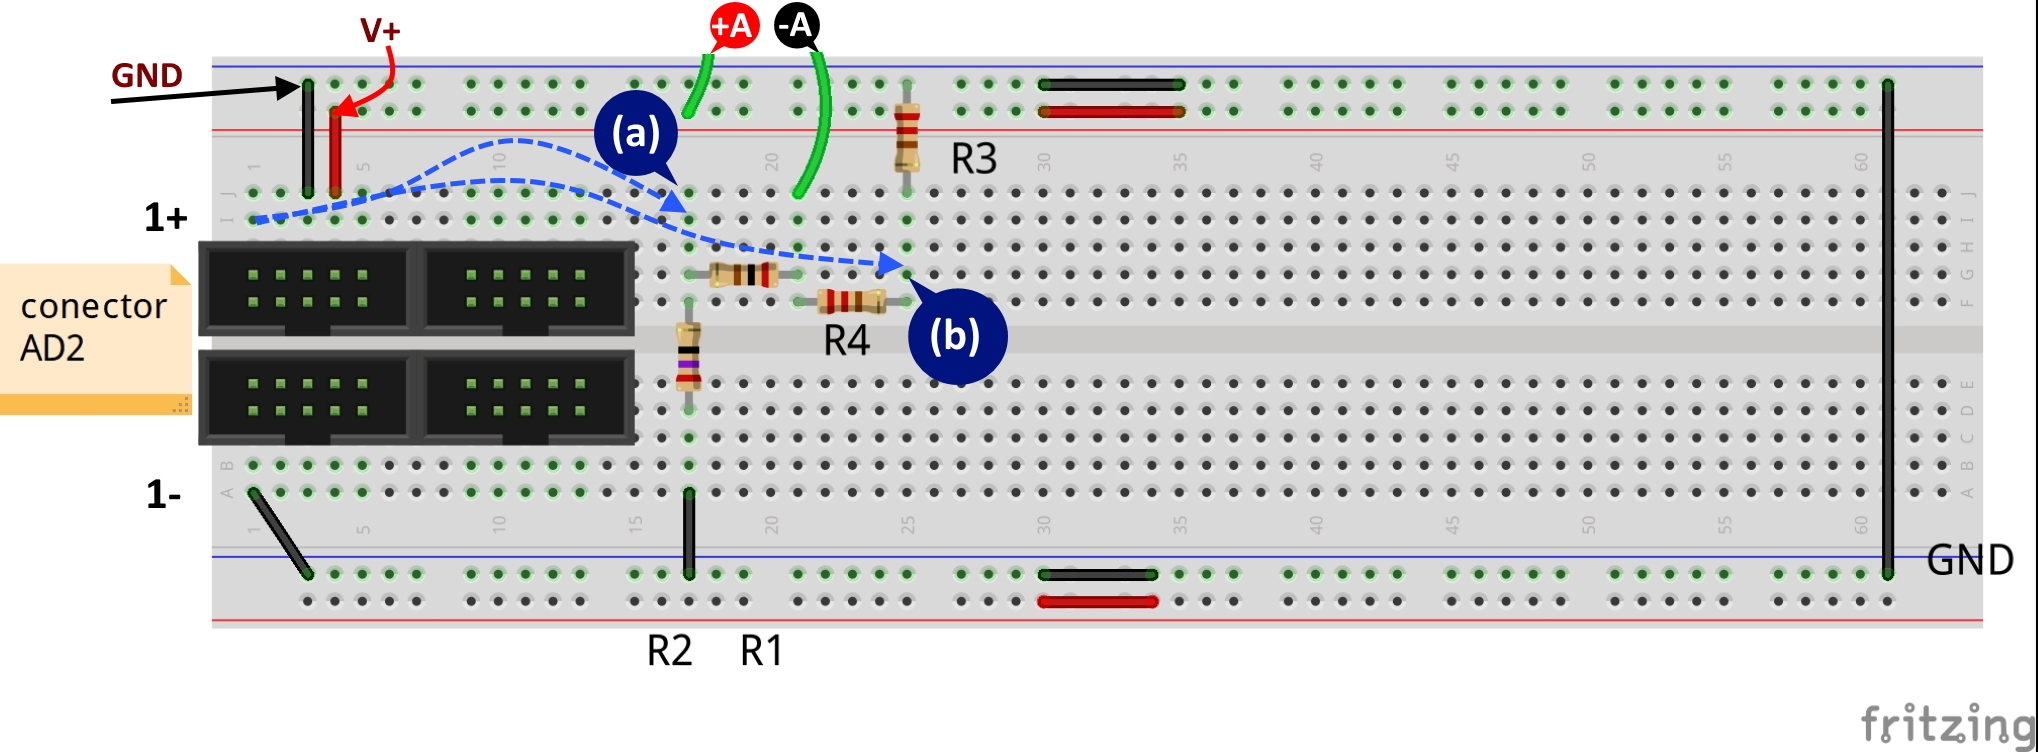
\includegraphics[width=0.8\textwidth]{laborator_01/figuri/4_punte_rez_bb}
	\caption{Montaj pentru m'asurarea parametrilor electrici de ie'sire ai pun'tii rezistive  'in sarcin'a.}
	\label{fig:4_punte_rez}
\end{figure}
%
% ---------------- Q10 -----------------
%
\begin{exercise} [Simularea modelului virtual al aplica'tiei] \label{Q10}
Folosind una din tehnicile descrise 'in sec'tiunea  \ref{sec:ltspice}, conform Fig.~\ref{fig:spice_ex1_3} 'si \ref{fig:spice_ex1_4}, simula'ti func'tionarea 'in sarcin'a a pun'tii rezistive construite. Completa'ti formularul de lucru cu rezultatele ob'tinute din simulare.
\end{exercise}
%
% ---------------- Q11 -----------------
%
\begin{exercise} [Caracteristici principale ale func'tion'arii aplica'tiei] \label{Q11}
Pentru acela'si montaj experimental de la exerci'tiul \ref{Q9} m'asura'ti tensiunea 'intre nodurile $(a)$ 'si $(b)$ ale pun'tii rezistive (Fig.~\ref{fig:4_punte_rez}). R'aspunde'ti cerin'telor specificate 'in formularul de lucru pentru acest exerci'tiu. 
\end{exercise}
%
% ---------------- Q12 -----------------
%
\begin{exercise} [Utiliz'ari ale aplica'tiei: m'asurarea de rezisten'te] \label{Q12}
Cea mai r'asp\^andit'a aplica'tie a pun'tii rezistive este cea de determinare de precizie a unor rezisten'te necunoscute; valorile necunoscute pot reprezenta rezisten'te ale unor rezistoare electrice liniare, sau rezisten'te ale unor senzori rezistivi a c'aror valoare este propor'tional'a cu m'arimi neelectrice (presiune, for't'a, temperatur'a, intensitate luminoas'a) m'asurate cu ajutorul acestor senzori. Exerci'tiul presupune m'asurarea rezisten'tei cunoscute a unui rezistor 'si compararea valorilor m'asurat'a 'si real'a. Urm'ari'ti pa'sii indica'ti 'in formularul de lucru pentru acest exerci'tiu. 
\end{exercise}
%
\begin{observ}
Rezisten'ta se m'asoar'a cu multimetrul setat pe scala de m'asur'a 2k;
\begin{itemize}
\item tensiunea $U_{ab}$ se determin'a cu ajutorul canalului de m'asur'a 1 al AD2, conect\^and nodurile (a) 'si (b) la bornele +1, respectiv -1 ale acestuia (v. fig. \ref{fig:4_punte_rez_x});
\item {\color{blue} Respecta'ti procedurile de lucru indicate la exerci'tiul \ref{Q5}; } 
\item  
	{\color{blue}
	Orice modificare 'in schem'a se va efectua fie cu portul USB al AD2 deconectat, fie cu sursele de tensiune oprite 
	("MASTER ENABLE" - 'in stare $\mathrm{OFF}$).}
\item Nota'ti-v'a pe foaia de calcul electronic'a rezultatele m'asur'arilor;
\end{itemize}
\end{observ}
%
\begin{indicatie}
'In Fig.~\ref{fig:4_punte_rez_x} este recomandat'a o posibil'a dispunere a componentelor.

Poten'tiometrul este o component'a rezistiv'a cu rezisten'ta variabil'a prin deplasarea rotativ'a sau liniar'a a unui contact mobil numit {\em cursor} 'intre dou'a contacte cu pozi'tie extrem'a: \textit{valoare 0}, respectiv \textit{valoare maxim'a}. Valoarea maxim'a este cea care caracterizeaza poten'tiometrul respectiv. Dac'a reglajul  nu este accesibil dec\^at limitat, direct pe placa de montaj, spunem c'a acest poten'tiometru este {\em semireglabil}. 
'In cazul 'in care cursorul formeaz'a un nod cu una din bornele extreme spunem c'a avem o {\em rezisten't'a variabil'a simpl'a}. 'In cazul 'in care cursorul este nelegat de contactele extreme, poten'tiometrul poate fi privit ca un divizor de tensiune, cu tensiunea de ie'sire reglabil'a 'intre 0 'si tensiunea aplicat'a 'intre bornele extreme, 'in func'tie de pozi'tia cursorului relativ la acestea din urm'a  (Fig. \ref{fig:potentiometru}).
\end{indicatie}

\newpage

\begin{figure}
	\centering
		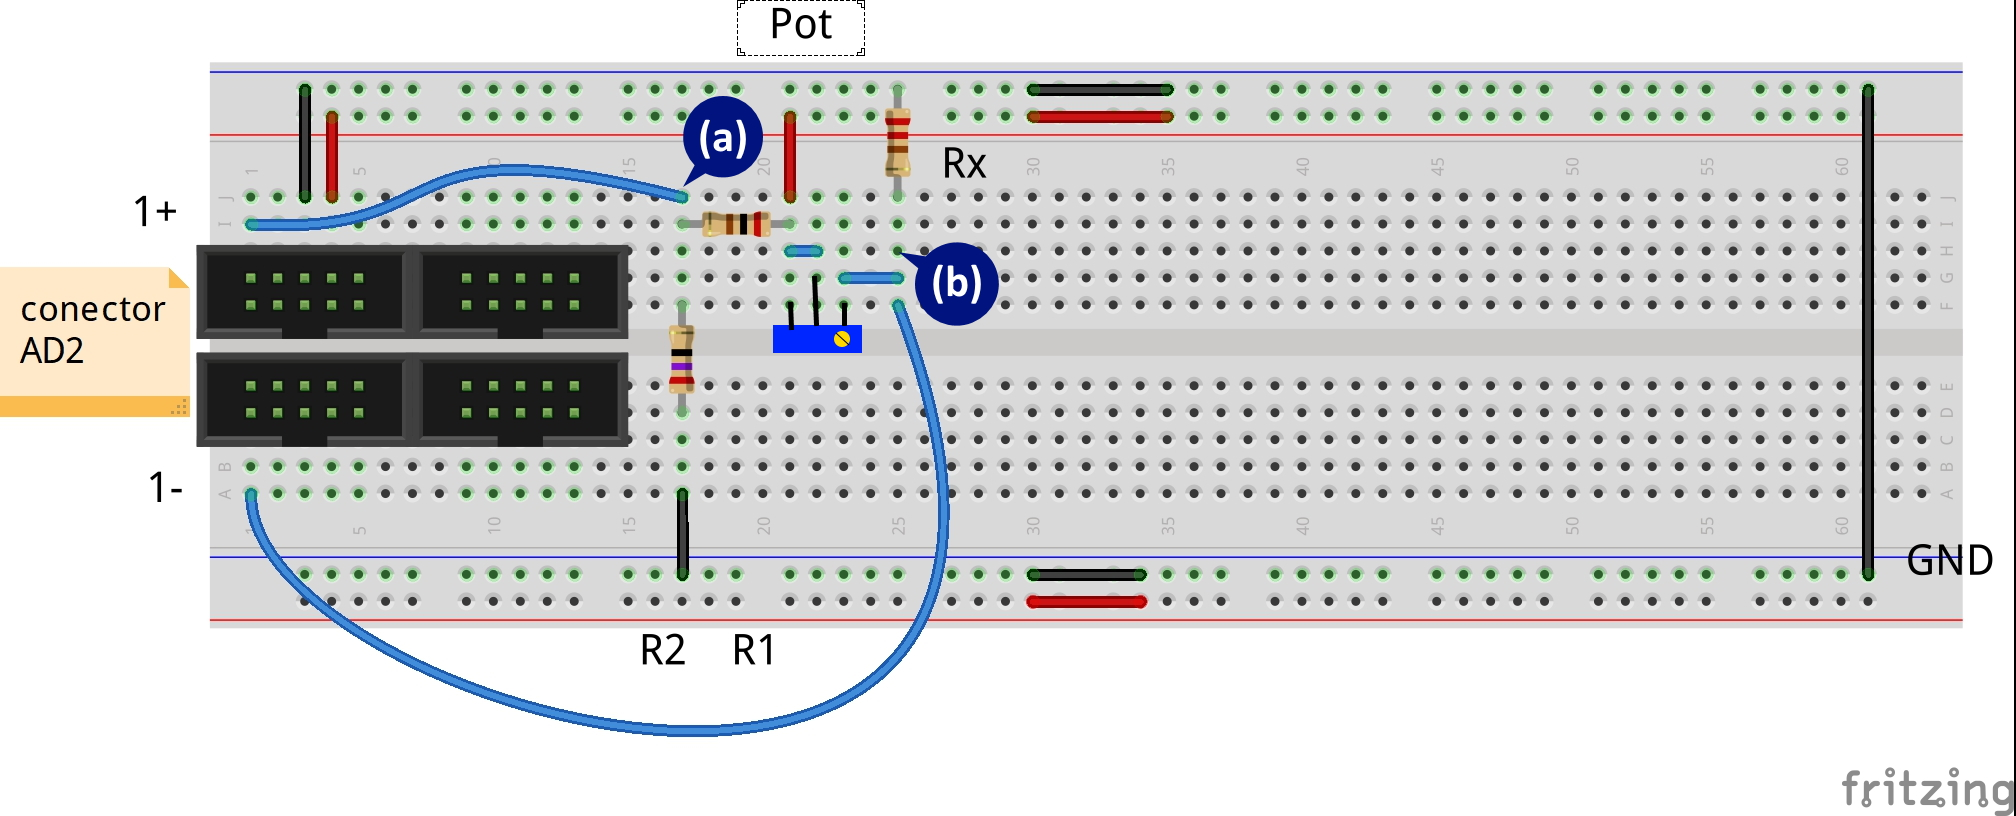
\includegraphics[width=0.8\textwidth]{laborator_01/figuri/4_punte_rez_x_bb}
	\caption{Montaj pentru m'asurarea unei rezisten'te necunoscute.}
	\label{fig:4_punte_rez_x}
%\end{figure}
%\begin{figure}
	\centering
		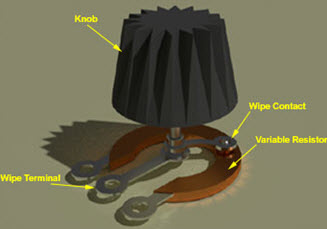
\includegraphics[width=0.35\textwidth]{laborator_01/figuri/6_potentiometru0}
		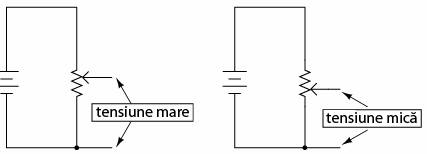
\includegraphics[width=0.45\textwidth]{laborator_01/figuri/6_potentiometru2}
	\caption{Poten'tiometrul. Tensiunea de ie'sire se modific'a 'in func'tie de pozi'tia cursorului 'intre bornele extreme. \cite{aplicatii_potentiometru}.}
	\label{fig:potentiometru}
\end{figure}
%


\begin{exercise}[Ultimul pas]
La finalul lucr'arii, revede'ti r'aspunsurile completate 'in chestionarul de laborator, finaliza'ti 'si 'inchide'ti chestionarul. Nota ob'tinut'a va fi afi'sat'a imediat.
\end{exercise}





